\documentclass[11pt,fleqn]{exam}

\setlength {\topmargin} {-.15in}
\setlength {\textheight} {8.6in}
\usepackage{enumerate}
\usepackage{amsmath}
\usepackage{amssymb}
\usepackage{xcolor}
\usepackage[colorlinks = true,
            linkcolor = blue,
            urlcolor  = blue,
            citecolor = blue,
            anchorcolor = blue]{hyperref}
\usepackage{listings}
\usepackage{color} %red, green, blue, yellow, cyan, magenta, black, white
\usepackage{graphicx}
\definecolor{mygreen}{RGB}{28,172,0} % color values Red, Green, Blue
\definecolor{mylilas}{RGB}{170,55,241}
\newcommand{\nn}{~\newline \noindent }
\newcommand{\mname}[1]{\mbox{\sf #1}}


\begin{document}

\lstset{language=Matlab,%
    %basicstyle=\color{red},
    breaklines=true,%
    morekeywords={matlab2tikz},
    keywordstyle=\color{blue},%
    morekeywords=[2]{1}, keywordstyle=[2]{\color{black}},
    identifierstyle=\color{black},%
    stringstyle=\color{mylilas},
    commentstyle=\color{mygreen},%
    showstringspaces=false,%without this there will be a symbol in the places where there is a space
    numbers=none,%
    numberstyle={\tiny \color{black}},% size of the numbers
    numbersep=9pt, % this defines how far the numbers are from the text
    emph=[1]{for,end,break},emphstyle=[1]\color{red}, %some words to emphasise
    %emph=[2]{word1,word2}, emphstyle=[2]{style},    
}
	
	\begin{center}
		
		{\large \textbf{COMPSCI 4X03}}\\[2mm]
		{\huge \textbf{Assignment 1}}\\[6mm]
		{\large \textbf{Mingzhe Wang}}\\[2mm]
		{\large \textbf{McMaster University}}\\[6mm]
		{\large \today}
		
	\end{center}
	
	\medskip
		
	\subsection*{Problems 1}
	\subsubsection*{q1}
	\lstinputlisting{q1.m}
	
	\nn
	\subsubsection*{output}
	\begin{lstlisting}
	9.600000e+01
	9.600000e+01
	9.600000e+01
	9.519604e+01
	9.600000e+01
	\end{lstlisting}
	
	\nn
	The accurate result should be $vpa(a) + vpa(b) + vpa(c) = vpa(a) + vpa(c) + vpa(b) = 9.519604e+01$. And only the $(a+c)+b$ equation calculate to this most accurate result. The reason is that by default, MATLB uses 16 digits of precision, which means when we calculate $a + b$ or $b + c$, due to the large difference between them (beyond 16 digit precision), the smaller number's precision is lost, which induces inaccuracy. However, by doing $(a+c)+b$, the $a+c$ part cancel a lot of digits because their digits are the same except the last one. Then the result ($a+c$) now becomes a small number, whose magnitude does not have a large difference with the b's.  Therefore, this method $(a+c)+b$ gives us the most accuracy result in this case.
	\subsection*{Problems 2}
	\begin{enumerate}[a.]
	\item If $a = 9.999 \times 10^1$, $b = 9.999 \times 10^1$, then $(a + b) / 2 = 1.000 \times 10^2 \not \in \{9.999\times10^1\}$.
	\item If $a = 1.234 \times 10^3$, $b = 4.547 \times 10^1$, $c = 0.004 \times 10^{-1}$, then $a + (b + c) = 1.280 \times 10^3 \neq 1.279 \times 10^3 = (a + b) + c$. 
	\item  If $a = 1.234 \times 10^3$, $b = 4.547 \times 10^1$, $c = 0.004 \times 10^{-1}$, then $a * (b * c) = 2.245 \times 10^1 \neq 2.244 \times 10^1 = (a * b) * c$. 
	\end{enumerate}
	

	\noindent No. By assumption $a < b$, we have $(a + b) / 2 < (b + b) / 2 = b$. In IEEE-754 FP system, for $x \leq y$, $fl(x) \leq fl(y)$, which is also the hint, so we have $fl( (a + b) / 2) \leq fl(b)$. Because $b$ is an IEEE-754 FP number, $fl(b) = b$. Therefore, $fl( (a + b) / 2) \leq b$. Similarly, we can show $a \leq fl( (a + b) / 2)$. Therefore $(a + b) / 2 \not \in [a, b]$ cannot occur.
	
	\subsection*{Problems 3}
	\subsubsection*{expsum1}
	\lstinputlisting{expsum1.m}
	
	\nn
	\subsubsection*{expsum2}
	\lstinputlisting{expsum2.m}
	
	\nn
	\subsubsection*{expsum3}
	\lstinputlisting{expsum3.m}
	
	\nn
	\subsubsection*{main\_expsum}
	\lstinputlisting{main_expsum.m}
	
	\nn
	\subsubsection*{output}
	\begin{lstlisting}
>> main_expsum
expsum1 result
   x     accurate value       approx.value     abs.error rel.error
-20.0  2.061153622439e-09  4.173637499438e-09  2.11e-09  1.02e+00 
-15.0  3.059023205018e-07  3.059054877425e-07  3.17e-12  1.04e-05 
 -5.0  6.737946999085e-03  6.737946999087e-03  1.44e-15  2.14e-13 
 -1.0  3.678794411714e-01  3.678794411714e-01  1.11e-16  3.02e-16 
  1.0  2.718281828459e+00  2.718281828459e+00  0.00e+00  0.00e+00 
  5.0  1.484131591026e+02  1.484131591026e+02  2.84e-14  1.92e-16 
 15.0  3.269017372472e+06  3.269017372472e+06  0.00e+00  0.00e+00 
 20.0  4.851651954098e+08  4.851651954098e+08  1.19e-07  2.46e-16 

expsum2 result
   x     accurate value       approx.value     abs.error rel.error
-20.0  2.061153622439e-09  2.061153622439e-09  4.14e-25  2.01e-16 
-15.0  3.059023205018e-07  3.059023205018e-07  0.00e+00  0.00e+00 
 -5.0  6.737946999085e-03  6.737946999085e-03  1.73e-18  2.57e-16 
 -1.0  3.678794411714e-01  3.678794411714e-01  5.55e-17  1.51e-16 
  1.0  2.718281828459e+00  2.718281828459e+00  0.00e+00  0.00e+00 
  5.0  1.484131591026e+02  1.484131591026e+02  2.84e-14  1.92e-16 
 15.0  3.269017372472e+06  3.269017372472e+06  0.00e+00  0.00e+00 
 20.0  4.851651954098e+08  4.851651954098e+08  1.19e-07  2.46e-16 

expsum3 result
   x     accurate value       approx.value     abs.error rel.error
-20.0  2.061153622439e-09  5.960464477539e-08  5.75e-08  2.79e+01 
-15.0  3.059023205018e-07  3.057066351175e-07  1.96e-10  6.40e-04 
 -5.0  6.737946999085e-03  6.737946999095e-03  9.89e-15  1.47e-12 
 -1.0  3.678794411714e-01  3.678794411714e-01  0.00e+00  0.00e+00 
  1.0  2.718281828459e+00  2.718281828459e+00  0.00e+00  0.00e+00 
  5.0  1.484131591026e+02  1.484131591026e+02  2.84e-14  1.92e-16 
 15.0  3.269017372472e+06  3.269017372472e+06  0.00e+00  0.00e+00 
 20.0  4.851651954098e+08  4.851651954098e+08  1.19e-07  2.46e-16 

	\end{lstlisting}


\nn \textbf{a.} As showed above, the accuracy (measured by relative error) of expsum1, expsum2, expsum3 for positive input is the same. While for negative input, expsum2 has the highest accuracy, expsum3 has the lowest accuracy, with expsum1 in the middle.  

\nn Note the methods are corresponding to the following equations:\\
\begin{align*}
e^x &= 1 + x + \frac{x^2}{2!} + \frac{x^3}{3!} + ...  \\
e^x &= \frac{1}{e^{-x}} = \frac{1}{1 + (-x) + \frac{x^2}{2!} + (-\frac{x^3}{3!}) + ...} \\
e^x &= \mname{pos\_terms} + \mname{neg\_terms} = (1 + \frac{x^2}{2!} + ... ) + (x + \frac{x^3}{3!} + ... )	   
\end{align*}

\nn For postive input, there is no cancellation error for all of this methods, because all the terms are positive. So the accuracy should be the same.

\nn However, for negtive input, note the second method doesn't have any cancellation error because all terms are positive, it has the highest accuracy. While the first method has cancellation error between each pair of even and odd terms, that's why its accuracy is the lowest. Finally, it seems the third equation doesn't have cancellation error either in $\mname{pos\_terms}$ or $\mname{neg\_terms}$, when the two sub-summations finally are added up, they also have cancellation error, because when the n is large enough, the two sub-sum should approaches the same abs value.\\

\nn \textbf{b.} No. As the above reasoning, even there is no cancellation error either in $\mname{pos\_terms}$ or $\mname{neg\_terms}$, when the two sub-summations are finally added up, they also have cancellation error, because when the n is large enough, the two sub-sum should approaches the same abs value with different signs. 

\subsection*{Problems 4}
\textbf{a.} \\
\lstset{language=bash}
\begin{lstlisting}
Memory required:  3914K.


LINPACK benchmark
Single precision
Digits:  6 
Array size 1000 X 1000.
Average rolled and unrolled performance:

    Reps Time(s) DGEFA   DGESL  OVERHEAD    MFLOPS     GFLOPS
-------------------------------------------------------------
       8   0.83  96.39%   0.00%   3.61%   1676.667      1.677
      16   1.68  95.83%   0.00%   4.17%   1666.253      1.666
      32   3.34  95.81%   0.30%   3.89%   1671.443      1.671
      64   6.69  95.37%   0.60%   4.04%   1671.443      1.671
     128  13.39  95.89%   0.22%   3.88%   1667.547      1.668

Memory required:  7824K.


LINPACK benchmark
Double precision
Digits:  15 
Array size 1000 X 1000.
Average rolled and unrolled performance:

    Reps Time(s) DGEFA   DGESL  OVERHEAD    MFLOPS     GFLOPS
-------------------------------------------------------------
       8   0.98  95.92%   0.00%   4.08%   1426.950      1.427
      16   1.94  97.42%   0.00%   2.58%   1419.400      1.419
      32   3.88  96.91%   0.52%   2.58%   1419.400      1.419
      64   7.77  97.04%   0.51%   2.45%   1415.655      1.416
     128  15.54  96.78%   0.51%   2.70%   1419.400      1.419

Memory required:  15645K.


LINPACK benchmark
LongDouble precision
Digits:  18 
Array size 1000 X 1000.
Average rolled and unrolled performance:

    Reps Time(s) DGEFA   DGESL  OVERHEAD    MFLOPS     GFLOPS
-------------------------------------------------------------
       2   0.67  98.51%   1.49%   0.00%    500.498      0.500
       4   1.35  97.04%   0.74%   2.22%    508.081      0.508
       8   2.69  98.88%   0.37%   0.74%    502.372      0.502
      16   5.38  97.58%   0.56%   1.86%    508.081      0.508
      32  10.77  98.24%   0.46%   1.30%    504.735      0.505

Memory required:  15645K.


LINPACK benchmark
Float128 precision
Digits:  0 
Array size 1000 X 1000.
Average rolled and unrolled performance:

    Reps Time(s) DGEFA   DGESL  OVERHEAD    MFLOPS     GFLOPS
-------------------------------------------------------------
       1  23.00  99.26%   0.61%   0.13%      7.299      0.007
       
\end{lstlisting}

\nn \textbf{b.}

\nn As the above result shows,  for respond speed, these data types has the following order (from the most fast to the most slower): single precision, double precision, long double precision, float128. In particular, for 8 times' respond, the comsumed time is 0.83s, 0.98s, 2.69s; and the giga float point operations performed are 1.677, 1.427, 0.502, separately. It should be noted that the float128 could only respond 1 time in 23.00 seconds, which causes only one line result is output because it is beyond the time limit.\\
\nn The above result shows that for longer precision data types, the float point operations on them will take longer time.

\newpage
\subsection*{Problems 5}
\textbf{a.}\\
\begin{figure}[hbt!]
  	\centering
  	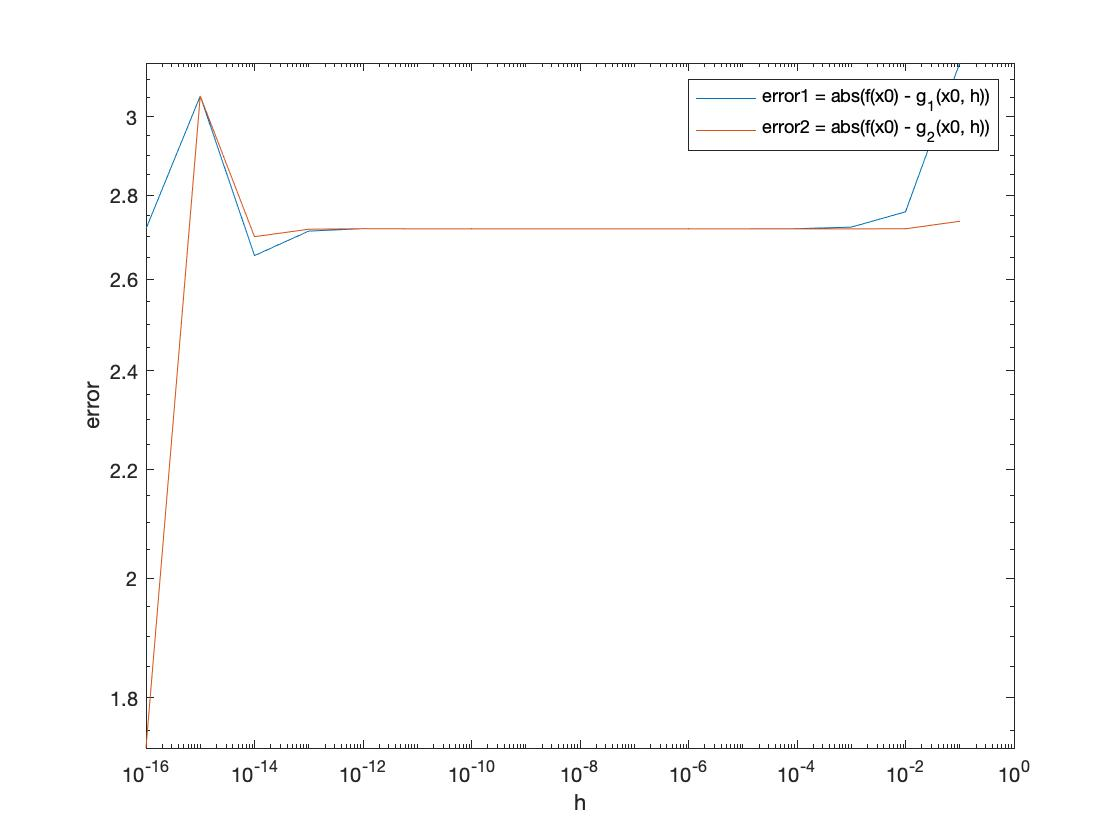
\includegraphics[width=1.0\textwidth]{loglog}
	\end{figure}

\nn \textbf{b.}\\
The minimum error1 is 2.655198e+00, which can be achieved by h = 1.000000e-14.\\
The minimum error2 is 1.722610e+00, which can be achieved by h = 1.000000e-16.

\nn \textbf{c.}\\
For error2, its truncation error is $O(h^2)$ and the original approximation can be simplified to the following:\\
\begin{equation*}
f'(x) \approx \frac{(1+h)e^{1+h} - (1-h)e^{1-h}}{2h}.
\end{equation*}
Note when $h \approx 0$, the cancellation error could appear. But also its truncation error will approaches 0, which could be able compensate the increasing of cancellation error. It should also be noted that the denominator part, compared with the error1's, is also has a coefficient of 2, which can also compensate the increasing of cancellation error. \\
The plot shows when $h$ is $1.000000e^{-16}$, which is the most nearest value of $h$ for all input $k$, the error2 is the smallest. Based on the above reasoning, this plot result is reasonable.

\nn For error1, its truncation error is $O(h)$ and the original approximation can be simplified to the following:\\
\begin{equation*}
f'(x) \approx \frac{(1+h)e^{1+h} - e}{h}.
\end{equation*}
Similarly, when $h \approx 0$, the cancellation error appears. However, compared to the error1: First, the domination's coefficient is 1, which has a lower contribution for compensating the increasing of cancellation error. Second, the because the truncation error is $O(h)$, which has a lower power than error1, when the $h \approx 0$, the decreasing truncation error also has a lower contribution for compensating the increasing of cancellation error. \\
The plot shows when $h$ is $1.000000e^{-14}$, which is the some value of $h$ for all input $k$, the error1 is the smallest.  This plot result is also reasonable based on the above reasoning, the point where $h = 1.000000e^{-14}$ should be somewhere the h value contributes the most to decreasing both the truncation and cancellation error.

\subsection*{Problems 6}
\lstset{language=Matlab,%
    %basicstyle=\color{red},
    breaklines=true,%
    morekeywords={matlab2tikz},
    keywordstyle=\color{blue},%
    morekeywords=[2]{1}, keywordstyle=[2]{\color{black}},
    identifierstyle=\color{black},%
    stringstyle=\color{mylilas},
    commentstyle=\color{mygreen},%
    showstringspaces=false,%without this there will be a symbol in the places where there is a space
    numbers=none,%
    numberstyle={\tiny \color{black}},% size of the numbers
    numbersep=9pt, % this defines how far the numbers are from the text
    emph=[1]{for,end,break},emphstyle=[1]\color{red}, %some words to emphasise
    %emph=[2]{word1,word2}, emphstyle=[2]{style},    
}

\subsubsection*{decSum}
\lstinputlisting{decSum.m}

\nn
\subsubsection*{incSum}
\lstinputlisting{incSum.m}

\nn
\subsubsection*{kahanSum}
\lstinputlisting{kahanSum.m}

\nn
\subsubsection*{accSum}
\lstinputlisting{accSum.m}

\nn
\subsubsection*{main\_Sum}
\lstinputlisting{main_Sum.m}

\nn
\subsection*{output}
\lstset{language=bash}
\begin{lstlisting}
>> main_sum
decreasing order      3.4063e-14
increasing order      3.2404e-15
Kahan's sum           3.1227e-16
\end{lstlisting}

\nn
\subsection*{Discussion}
As the result shows, the Kahan's summation algorithm is the most accurate way to compute this sum.  The error in the summation is raised by the fact that when adding a small number (each term) to a large number (sum result),  we loss information (the lower bit of small number), which induces the error. So decreasing order summation has the worst accuracy because when as the index grows, the difference between sum result and each term also grows, and the last terms could even be omitted. 

\nn Kahan's summation algorithm is the most accuracy way by using a correction factor c to automatically correct the sum result during the summation process. It's process can be illustrated by the following diagram, which I found from the Oracle's document. (\href{https://docs.oracle.com/cd/E19957-01/806-3568/ncg_goldberg.html}{What Every Computer Scientist Should Know About Floating-Point Arithmeti}.)\\

\begin{figure}[hbt!]
  	\centering
  	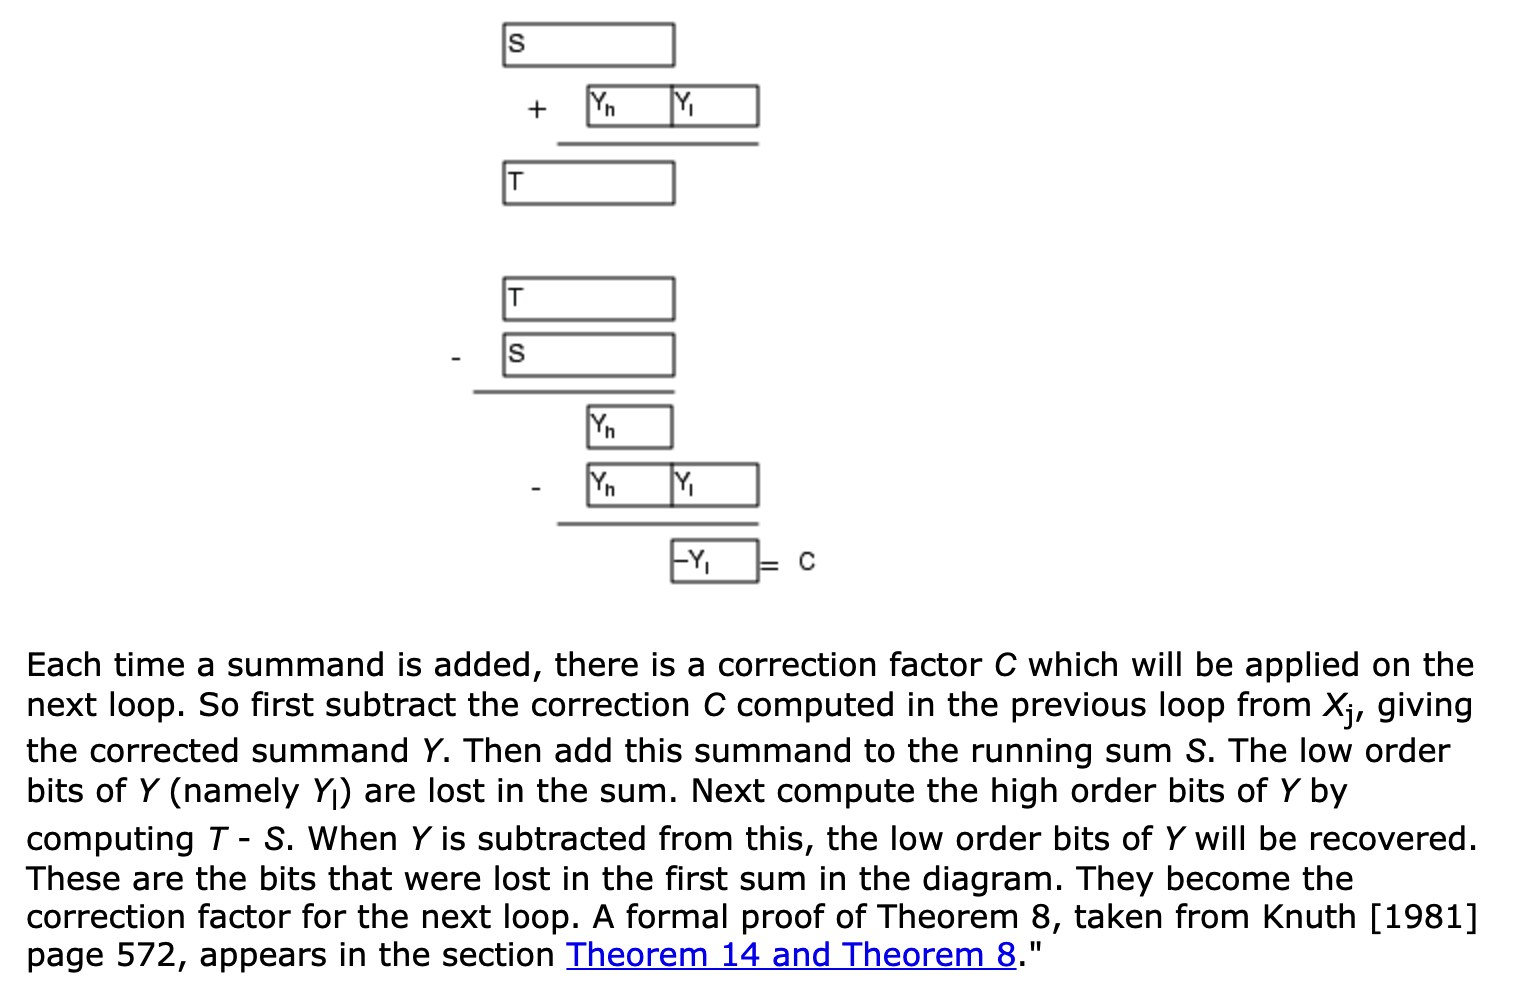
\includegraphics[width=1.0\textwidth]{kahanSum}
\end{figure}




\end{document}


